%%%%%%%%%%%%%%%%%%%%%%%%%%%%%% -*- Mode: Latex -*- %%%%%%%%%%%%%%%%%%%%%%%%%%%%
%% 03-01.tex -- JBlanket ICSE Paper
%% Author          : Philip Johnson
%% Created On      : Mon Sep 23 11:52:28 2002
%% Last Modified By: Philip M. Johnson
%% Last Modified On: Mon Sep 22 10:00:22 2003
%% RCS: $Id$
%%%%%%%%%%%%%%%%%%%%%%%%%%%%%%%%%%%%%%%%%%%%%%%%%%%%%%%%%%%%%%%%%%%%%%%%%%%%%%%
%%   Copyright (C) 2002 Philip Johnson
%%%%%%%%%%%%%%%%%%%%%%%%%%%%%%%%%%%%%%%%%%%%%%%%%%%%%%%%%%%%%%%%%%%%%%%%%%%%%%%
%% 

\documentclass[10pt,twocolumn]{article} 
% Psfig/TeX 
\def\PsfigVersion{1.9}
% dvips version
%
% All psfig/tex software, documentation, and related files
% in this distribution of psfig/tex are 
% Copyright 1987, 1988, 1991 Trevor J. Darrell
%
% Permission is granted for use and non-profit distribution of psfig/tex 
% providing that this notice is clearly maintained. The right to
% distribute any portion of psfig/tex for profit or as part of any commercial
% product is specifically reserved for the author(s) of that portion.
%
% *** Feel free to make local modifications of psfig as you wish,
% *** but DO NOT post any changed or modified versions of ``psfig''
% *** directly to the net. Send them to me and I'll try to incorporate
% *** them into future versions. If you want to take the psfig code 
% *** and make a new program (subject to the copyright above), distribute it, 
% *** (and maintain it) that's fine, just don't call it psfig.
%
% Bugs and improvements to trevor@media.mit.edu.
%
% Thanks to Greg Hager (GDH) and Ned Batchelder for their contributions
% to the original version of this project.
%
% Modified by J. Daniel Smith on 9 October 1990 to accept the
% %%BoundingBox: comment with or without a space after the colon.  Stole
% file reading code from Tom Rokicki's EPSF.TEX file (see below).
%
% More modifications by J. Daniel Smith on 29 March 1991 to allow the
% the included PostScript figure to be rotated.  The amount of
% rotation is specified by the "angle=" parameter of the \psfig command.
%
% Modified by Robert Russell on June 25, 1991 to allow users to specify
% .ps filenames which don't yet exist, provided they explicitly provide
% boundingbox information via the \psfig command. Note: This will only work
% if the "file=" parameter follows all four "bb???=" parameters in the
% command. This is due to the order in which psfig interprets these params.
%
%  3 Jul 1991	JDS	check if file already read in once
%  4 Sep 1991	JDS	fixed incorrect computation of rotated
%			bounding box
% 25 Sep 1991	GVR	expanded synopsis of \psfig
% 14 Oct 1991	JDS	\fbox code from LaTeX so \psdraft works with TeX
%			changed \typeout to \ps@typeout
% 17 Oct 1991	JDS	added \psscalefirst and \psrotatefirst
%

% From: gvr@cs.brown.edu (George V. Reilly)
%
% \psdraft	draws an outline box, but doesn't include the figure
%		in the DVI file.  Useful for previewing.
%
% \psfull	includes the figure in the DVI file (default).
%
% \psscalefirst width= or height= specifies the size of the figure
% 		before rotation.
% \psrotatefirst (default) width= or height= specifies the size of the
% 		 figure after rotation.  Asymetric figures will
% 		 appear to shrink.
%
% \psfigurepath#1	sets the path to search for the figure
%
% \psfig
% usage: \psfig{file=, figure=, height=, width=,
%			bbllx=, bblly=, bburx=, bbury=,
%			rheight=, rwidth=, clip=, angle=, silent=}
%
%	"file" is the filename.  If no path name is specified and the
%		file is not found in the current directory,
%		it will be looked for in directory \psfigurepath.
%	"figure" is a synonym for "file".
%	By default, the width and height of the figure are taken from
%		the BoundingBox of the figure.
%	If "width" is specified, the figure is scaled so that it has
%		the specified width.  Its height changes proportionately.
%	If "height" is specified, the figure is scaled so that it has
%		the specified height.  Its width changes proportionately.
%	If both "width" and "height" are specified, the figure is scaled
%		anamorphically.
%	"bbllx", "bblly", "bburx", and "bbury" control the PostScript
%		BoundingBox.  If these four values are specified
%               *before* the "file" option, the PSFIG will not try to
%               open the PostScript file.
%	"rheight" and "rwidth" are the reserved height and width
%		of the figure, i.e., how big TeX actually thinks
%		the figure is.  They default to "width" and "height".
%	The "clip" option ensures that no portion of the figure will
%		appear outside its BoundingBox.  "clip=" is a switch and
%		takes no value, but the `=' must be present.
%	The "angle" option specifies the angle of rotation (degrees, ccw).
%	The "silent" option makes \psfig work silently.
%

% check to see if macros already loaded in (maybe some other file says
% "\input psfig") ...
\ifx\undefined\psfig\else\endinput\fi

%
% from a suggestion by eijkhout@csrd.uiuc.edu to allow
% loading as a style file. Changed to avoid problems
% with amstex per suggestion by jbence@math.ucla.edu

\let\LaTeXAtSign=\@
\let\@=\relax
\edef\psfigRestoreAt{\catcode`\@=\number\catcode`@\relax}
%\edef\psfigRestoreAt{\catcode`@=\number\catcode`@\relax}
\catcode`\@=11\relax
\newwrite\@unused
\def\ps@typeout#1{{\let\protect\string\immediate\write\@unused{#1}}}
\ps@typeout{psfig/tex \PsfigVersion}

%% Here's how you define your figure path.  Should be set up with null
%% default and a user useable definition.

\def\figurepath{./}
\def\psfigurepath#1{\edef\figurepath{#1}}

%
% @psdo control structure -- similar to Latex @for.
% I redefined these with different names so that psfig can
% be used with TeX as well as LaTeX, and so that it will not 
% be vunerable to future changes in LaTeX's internal
% control structure,
%
\def\@nnil{\@nil}
\def\@empty{}
\def\@psdonoop#1\@@#2#3{}
\def\@psdo#1:=#2\do#3{\edef\@psdotmp{#2}\ifx\@psdotmp\@empty \else
    \expandafter\@psdoloop#2,\@nil,\@nil\@@#1{#3}\fi}
\def\@psdoloop#1,#2,#3\@@#4#5{\def#4{#1}\ifx #4\@nnil \else
       #5\def#4{#2}\ifx #4\@nnil \else#5\@ipsdoloop #3\@@#4{#5}\fi\fi}
\def\@ipsdoloop#1,#2\@@#3#4{\def#3{#1}\ifx #3\@nnil 
       \let\@nextwhile=\@psdonoop \else
      #4\relax\let\@nextwhile=\@ipsdoloop\fi\@nextwhile#2\@@#3{#4}}
\def\@tpsdo#1:=#2\do#3{\xdef\@psdotmp{#2}\ifx\@psdotmp\@empty \else
    \@tpsdoloop#2\@nil\@nil\@@#1{#3}\fi}
\def\@tpsdoloop#1#2\@@#3#4{\def#3{#1}\ifx #3\@nnil 
       \let\@nextwhile=\@psdonoop \else
      #4\relax\let\@nextwhile=\@tpsdoloop\fi\@nextwhile#2\@@#3{#4}}
% 
% \fbox is defined in latex.tex; so if \fbox is undefined, assume that
% we are not in LaTeX.
% Perhaps this could be done better???
\ifx\undefined\fbox
% \fbox code from modified slightly from LaTeX
\newdimen\fboxrule
\newdimen\fboxsep
\newdimen\ps@tempdima
\newbox\ps@tempboxa
\fboxsep = 3pt
\fboxrule = .4pt
\long\def\fbox#1{\leavevmode\setbox\ps@tempboxa\hbox{#1}\ps@tempdima\fboxrule
    \advance\ps@tempdima \fboxsep \advance\ps@tempdima \dp\ps@tempboxa
   \hbox{\lower \ps@tempdima\hbox
  {\vbox{\hrule height \fboxrule
          \hbox{\vrule width \fboxrule \hskip\fboxsep
          \vbox{\vskip\fboxsep \box\ps@tempboxa\vskip\fboxsep}\hskip 
                 \fboxsep\vrule width \fboxrule}
                 \hrule height \fboxrule}}}}
\fi
%
%%%%%%%%%%%%%%%%%%%%%%%%%%%%%%%%%%%%%%%%%%%%%%%%%%%%%%%%%%%%%%%%%%%
% file reading stuff from epsf.tex
%   EPSF.TEX macro file:
%   Written by Tomas Rokicki of Radical Eye Software, 29 Mar 1989.
%   Revised by Don Knuth, 3 Jan 1990.
%   Revised by Tomas Rokicki to accept bounding boxes with no
%      space after the colon, 18 Jul 1990.
%   Portions modified/removed for use in PSFIG package by
%      J. Daniel Smith, 9 October 1990.
%
\newread\ps@stream
\newif\ifnot@eof       % continue looking for the bounding box?
\newif\if@noisy        % report what you're making?
\newif\if@atend        % %%BoundingBox: has (at end) specification
\newif\if@psfile       % does this look like a PostScript file?
%
% PostScript files should start with `%!'
%
{\catcode`\%=12\global\gdef\epsf@start{%!}}
\def\epsf@PS{PS}
%
\def\epsf@getbb#1{%
%
%   The first thing we need to do is to open the
%   PostScript file, if possible.
%
\openin\ps@stream=#1
\ifeof\ps@stream\ps@typeout{Error, File #1 not found}\else
%
%   Okay, we got it. Now we'll scan lines until we find one that doesn't
%   start with %. We're looking for the bounding box comment.
%
   {\not@eoftrue \chardef\other=12
    \def\do##1{\catcode`##1=\other}\dospecials \catcode`\ =10
    \loop
       \if@psfile
	  \read\ps@stream to \epsf@fileline
       \else{
	  \obeyspaces
          \read\ps@stream to \epsf@tmp\global\let\epsf@fileline\epsf@tmp}
       \fi
       \ifeof\ps@stream\not@eoffalse\else
%
%   Check the first line for `%!'.  Issue a warning message if its not
%   there, since the file might not be a PostScript file.
%
       \if@psfile\else
       \expandafter\epsf@test\epsf@fileline:. \\%
       \fi
%
%   We check to see if the first character is a % sign;
%   if so, we look further and stop only if the line begins with
%   `%%BoundingBox:' and the `(atend)' specification was not found.
%   That is, the only way to stop is when the end of file is reached,
%   or a `%%BoundingBox: llx lly urx ury' line is found.
%
          \expandafter\epsf@aux\epsf@fileline:. \\%
       \fi
   \ifnot@eof\repeat
   }\closein\ps@stream\fi}%
%
% This tests if the file we are reading looks like a PostScript file.
%
\long\def\epsf@test#1#2#3:#4\\{\def\epsf@testit{#1#2}
			\ifx\epsf@testit\epsf@start\else
\ps@typeout{Warning! File does not start with `\epsf@start'.  It may not be a PostScript file.}
			\fi
			\@psfiletrue} % don't test after 1st line
%
%   We still need to define the tricky \epsf@aux macro. This requires
%   a couple of magic constants for comparison purposes.
%
{\catcode`\%=12\global\let\epsf@percent=%\global\def\epsf@bblit{%BoundingBox}}
%
%
%   So we're ready to check for `%BoundingBox:' and to grab the
%   values if they are found.  We continue searching if `(at end)'
%   was found after the `%BoundingBox:'.
%
\long\def\epsf@aux#1#2:#3\\{\ifx#1\epsf@percent
   \def\epsf@testit{#2}\ifx\epsf@testit\epsf@bblit
	\@atendfalse
        \epsf@atend #3 . \\%
	\if@atend	
	   \if@verbose{
		\ps@typeout{psfig: found `(atend)'; continuing search}
	   }\fi
        \else
        \epsf@grab #3 . . . \\%
        \not@eoffalse
        \global\no@bbfalse
        \fi
   \fi\fi}%
%
%   Here we grab the values and stuff them in the appropriate definitions.
%
\def\epsf@grab #1 #2 #3 #4 #5\\{%
   \global\def\epsf@llx{#1}\ifx\epsf@llx\empty
      \epsf@grab #2 #3 #4 #5 .\\\else
   \global\def\epsf@lly{#2}%
   \global\def\epsf@urx{#3}\global\def\epsf@ury{#4}\fi}%
%
% Determine if the stuff following the %%BoundingBox is `(atend)'
% J. Daniel Smith.  Copied from \epsf@grab above.
%
\def\epsf@atendlit{(atend)} 
\def\epsf@atend #1 #2 #3\\{%
   \def\epsf@tmp{#1}\ifx\epsf@tmp\empty
      \epsf@atend #2 #3 .\\\else
   \ifx\epsf@tmp\epsf@atendlit\@atendtrue\fi\fi}


% End of file reading stuff from epsf.tex
%%%%%%%%%%%%%%%%%%%%%%%%%%%%%%%%%%%%%%%%%%%%%%%%%%%%%%%%%%%%%%%%%%%

%%%%%%%%%%%%%%%%%%%%%%%%%%%%%%%%%%%%%%%%%%%%%%%%%%%%%%%%%%%%%%%%%%%
% trigonometry stuff from "trig.tex"
\chardef\psletter = 11 % won't conflict with \begin{letter} now...
\chardef\other = 12

\newif \ifdebug %%% turn me on to see TeX hard at work ...
\newif\ifc@mpute %%% don't need to compute some values
\c@mputetrue % but assume that we do

\let\then = \relax
\def\r@dian{pt }
\let\r@dians = \r@dian
\let\dimensionless@nit = \r@dian
\let\dimensionless@nits = \dimensionless@nit
\def\internal@nit{sp }
\let\internal@nits = \internal@nit
\newif\ifstillc@nverging
\def \Mess@ge #1{\ifdebug \then \message {#1} \fi}

{ %%% Things that need abnormal catcodes %%%
	\catcode `\@ = \psletter
	\gdef \nodimen {\expandafter \n@dimen \the \dimen}
	\gdef \term #1 #2 #3%
	       {\edef \t@ {\the #1}%%% freeze parameter 1 (count, by value)
		\edef \t@@ {\expandafter \n@dimen \the #2\r@dian}%
				   %%% freeze parameter 2 (dimen, by value)
		\t@rm {\t@} {\t@@} {#3}%
	       }
	\gdef \t@rm #1 #2 #3%
	       {{%
		\count 0 = 0
		\dimen 0 = 1 \dimensionless@nit
		\dimen 2 = #2\relax
		\Mess@ge {Calculating term #1 of \nodimen 2}%
		\loop
		\ifnum	\count 0 < #1
		\then	\advance \count 0 by 1
			\Mess@ge {Iteration \the \count 0 \space}%
			\Multiply \dimen 0 by {\dimen 2}%
			\Mess@ge {After multiplication, term = \nodimen 0}%
			\Divide \dimen 0 by {\count 0}%
			\Mess@ge {After division, term = \nodimen 0}%
		\repeat
		\Mess@ge {Final value for term #1 of 
				\nodimen 2 \space is \nodimen 0}%
		\xdef \Term {#3 = \nodimen 0 \r@dians}%
		\aftergroup \Term
	       }}
	\catcode `\p = \other
	\catcode `\t = \other
	\gdef \n@dimen #1pt{#1} %%% throw away the ``pt''
}

\def \Divide #1by #2{\divide #1 by #2} %%% just a synonym

\def \Multiply #1by #2%%% allows division of a dimen by a dimen
       {{%%% should really freeze parameter 2 (dimen, passed by value)
	\count 0 = #1\relax
	\count 2 = #2\relax
	\count 4 = 65536
	\Mess@ge {Before scaling, count 0 = \the \count 0 \space and
			count 2 = \the \count 2}%
	\ifnum	\count 0 > 32767 %%% do our best to avoid overflow
	\then	\divide \count 0 by 4
		\divide \count 4 by 4
	\else	\ifnum	\count 0 < -32767
		\then	\divide \count 0 by 4
			\divide \count 4 by 4
		\else
		\fi
	\fi
	\ifnum	\count 2 > 32767 %%% while retaining reasonable accuracy
	\then	\divide \count 2 by 4
		\divide \count 4 by 4
	\else	\ifnum	\count 2 < -32767
		\then	\divide \count 2 by 4
			\divide \count 4 by 4
		\else
		\fi
	\fi
	\multiply \count 0 by \count 2
	\divide \count 0 by \count 4
	\xdef \product {#1 = \the \count 0 \internal@nits}%
	\aftergroup \product
       }}

\def\r@duce{\ifdim\dimen0 > 90\r@dian \then   % sin(x+90) = sin(180-x)
		\multiply\dimen0 by -1
		\advance\dimen0 by 180\r@dian
		\r@duce
	    \else \ifdim\dimen0 < -90\r@dian \then  % sin(-x) = sin(360+x)
		\advance\dimen0 by 360\r@dian
		\r@duce
		\fi
	    \fi}

\def\Sine#1%
       {{%
	\dimen 0 = #1 \r@dian
	\r@duce
	\ifdim\dimen0 = -90\r@dian \then
	   \dimen4 = -1\r@dian
	   \c@mputefalse
	\fi
	\ifdim\dimen0 = 90\r@dian \then
	   \dimen4 = 1\r@dian
	   \c@mputefalse
	\fi
	\ifdim\dimen0 = 0\r@dian \then
	   \dimen4 = 0\r@dian
	   \c@mputefalse
	\fi
%
	\ifc@mpute \then
        	% convert degrees to radians
		\divide\dimen0 by 180
		\dimen0=3.141592654\dimen0
%
		\dimen 2 = 3.1415926535897963\r@dian %%% a well-known constant
		\divide\dimen 2 by 2 %%% we only deal with -pi/2 : pi/2
		\Mess@ge {Sin: calculating Sin of \nodimen 0}%
		\count 0 = 1 %%% see power-series expansion for sine
		\dimen 2 = 1 \r@dian %%% ditto
		\dimen 4 = 0 \r@dian %%% ditto
		\loop
			\ifnum	\dimen 2 = 0 %%% then we've done
			\then	\stillc@nvergingfalse 
			\else	\stillc@nvergingtrue
			\fi
			\ifstillc@nverging %%% then calculate next term
			\then	\term {\count 0} {\dimen 0} {\dimen 2}%
				\advance \count 0 by 2
				\count 2 = \count 0
				\divide \count 2 by 2
				\ifodd	\count 2 %%% signs alternate
				\then	\advance \dimen 4 by \dimen 2
				\else	\advance \dimen 4 by -\dimen 2
				\fi
		\repeat
	\fi		
			\xdef \sine {\nodimen 4}%
       }}

% Now the Cosine can be calculated easily by calling \Sine
\def\Cosine#1{\ifx\sine\UnDefined\edef\Savesine{\relax}\else
		             \edef\Savesine{\sine}\fi
	{\dimen0=#1\r@dian\advance\dimen0 by 90\r@dian
	 \Sine{\nodimen 0}
	 \xdef\cosine{\sine}
	 \xdef\sine{\Savesine}}}	      
% end of trig stuff
%%%%%%%%%%%%%%%%%%%%%%%%%%%%%%%%%%%%%%%%%%%%%%%%%%%%%%%%%%%%%%%%%%%%

\def\psdraft{
	\def\@psdraft{0}
	%\ps@typeout{draft level now is \@psdraft \space . }
}
\def\psfull{
	\def\@psdraft{100}
	%\ps@typeout{draft level now is \@psdraft \space . }
}

\psfull

\newif\if@scalefirst
\def\psscalefirst{\@scalefirsttrue}
\def\psrotatefirst{\@scalefirstfalse}
\psrotatefirst

\newif\if@draftbox
\def\psnodraftbox{
	\@draftboxfalse
}
\def\psdraftbox{
	\@draftboxtrue
}
\@draftboxtrue

\newif\if@prologfile
\newif\if@postlogfile
\def\pssilent{
	\@noisyfalse
}
\def\psnoisy{
	\@noisytrue
}
\psnoisy
%%% These are for the option list.
%%% A specification of the form a = b maps to calling \@p@@sa{b}
\newif\if@bbllx
\newif\if@bblly
\newif\if@bburx
\newif\if@bbury
\newif\if@height
\newif\if@width
\newif\if@rheight
\newif\if@rwidth
\newif\if@angle
\newif\if@clip
\newif\if@verbose
\def\@p@@sclip#1{\@cliptrue}


\newif\if@decmpr

%%% GDH 7/26/87 -- changed so that it first looks in the local directory,
%%% then in a specified global directory for the ps file.
%%% RPR 6/25/91 -- changed so that it defaults to user-supplied name if
%%% boundingbox info is specified, assuming graphic will be created by
%%% print time.
%%% TJD 10/19/91 -- added bbfile vs. file distinction, and @decmpr flag

\def\@p@@sfigure#1{\def\@p@sfile{null}\def\@p@sbbfile{null}
	        \openin1=#1.bb
		\ifeof1\closein1
	        	\openin1=\figurepath#1.bb
			\ifeof1\closein1
			        \openin1=#1
				\ifeof1\closein1%
				       \openin1=\figurepath#1
					\ifeof1
					   \ps@typeout{Error, File #1 not found}
						\if@bbllx\if@bblly
				   		\if@bburx\if@bbury
			      				\def\@p@sfile{#1}%
			      				\def\@p@sbbfile{#1}%
							\@decmprfalse
				  	   	\fi\fi\fi\fi
					\else\closein1
				    		\def\@p@sfile{\figurepath#1}%
				    		\def\@p@sbbfile{\figurepath#1}%
						\@decmprfalse
	                       		\fi%
			 	\else\closein1%
					\def\@p@sfile{#1}
					\def\@p@sbbfile{#1}
					\@decmprfalse
			 	\fi
			\else
				\def\@p@sfile{\figurepath#1}
				\def\@p@sbbfile{\figurepath#1.bb}
				\@decmprtrue
			\fi
		\else
			\def\@p@sfile{#1}
			\def\@p@sbbfile{#1.bb}
			\@decmprtrue
		\fi}

\def\@p@@sfile#1{\@p@@sfigure{#1}}

\def\@p@@sbbllx#1{
		%\ps@typeout{bbllx is #1}
		\@bbllxtrue
		\dimen100=#1
		\edef\@p@sbbllx{\number\dimen100}
}
\def\@p@@sbblly#1{
		%\ps@typeout{bblly is #1}
		\@bbllytrue
		\dimen100=#1
		\edef\@p@sbblly{\number\dimen100}
}
\def\@p@@sbburx#1{
		%\ps@typeout{bburx is #1}
		\@bburxtrue
		\dimen100=#1
		\edef\@p@sbburx{\number\dimen100}
}
\def\@p@@sbbury#1{
		%\ps@typeout{bbury is #1}
		\@bburytrue
		\dimen100=#1
		\edef\@p@sbbury{\number\dimen100}
}
\def\@p@@sheight#1{
		\@heighttrue
		\dimen100=#1
   		\edef\@p@sheight{\number\dimen100}
		%\ps@typeout{Height is \@p@sheight}
}
\def\@p@@swidth#1{
		%\ps@typeout{Width is #1}
		\@widthtrue
		\dimen100=#1
		\edef\@p@swidth{\number\dimen100}
}
\def\@p@@srheight#1{
		%\ps@typeout{Reserved height is #1}
		\@rheighttrue
		\dimen100=#1
		\edef\@p@srheight{\number\dimen100}
}
\def\@p@@srwidth#1{
		%\ps@typeout{Reserved width is #1}
		\@rwidthtrue
		\dimen100=#1
		\edef\@p@srwidth{\number\dimen100}
}
\def\@p@@sangle#1{
		%\ps@typeout{Rotation is #1}
		\@angletrue
%		\dimen100=#1
		\edef\@p@sangle{#1} %\number\dimen100}
}
\def\@p@@ssilent#1{ 
		\@verbosefalse
}
\def\@p@@sprolog#1{\@prologfiletrue\def\@prologfileval{#1}}
\def\@p@@spostlog#1{\@postlogfiletrue\def\@postlogfileval{#1}}
\def\@cs@name#1{\csname #1\endcsname}
\def\@setparms#1=#2,{\@cs@name{@p@@s#1}{#2}}
%
% initialize the defaults (size the size of the figure)
%
\def\ps@init@parms{
		\@bbllxfalse \@bbllyfalse
		\@bburxfalse \@bburyfalse
		\@heightfalse \@widthfalse
		\@rheightfalse \@rwidthfalse
		\def\@p@sbbllx{}\def\@p@sbblly{}
		\def\@p@sbburx{}\def\@p@sbbury{}
		\def\@p@sheight{}\def\@p@swidth{}
		\def\@p@srheight{}\def\@p@srwidth{}
		\def\@p@sangle{0}
		\def\@p@sfile{} \def\@p@sbbfile{}
		\def\@p@scost{10}
		\def\@sc{}
		\@prologfilefalse
		\@postlogfilefalse
		\@clipfalse
		\if@noisy
			\@verbosetrue
		\else
			\@verbosefalse
		\fi
}
%
% Go through the options setting things up.
%
\def\parse@ps@parms#1{
	 	\@psdo\@psfiga:=#1\do
		   {\expandafter\@setparms\@psfiga,}}
%
% Compute bb height and width
%
\newif\ifno@bb
\def\bb@missing{
	\if@verbose{
		\ps@typeout{psfig: searching \@p@sbbfile \space  for bounding box}
	}\fi
	\no@bbtrue
	\epsf@getbb{\@p@sbbfile}
        \ifno@bb \else \bb@cull\epsf@llx\epsf@lly\epsf@urx\epsf@ury\fi
}	
\def\bb@cull#1#2#3#4{
	\dimen100=#1 bp\edef\@p@sbbllx{\number\dimen100}
	\dimen100=#2 bp\edef\@p@sbblly{\number\dimen100}
	\dimen100=#3 bp\edef\@p@sbburx{\number\dimen100}
	\dimen100=#4 bp\edef\@p@sbbury{\number\dimen100}
	\no@bbfalse
}
% rotate point (#1,#2) about (0,0).
% The sine and cosine of the angle are already stored in \sine and
% \cosine.  The result is placed in (\p@intvaluex, \p@intvaluey).
\newdimen\p@intvaluex
\newdimen\p@intvaluey
\def\rotate@#1#2{{\dimen0=#1 sp\dimen1=#2 sp
%            	calculate x' = x \cos\theta - y \sin\theta
		  \global\p@intvaluex=\cosine\dimen0
		  \dimen3=\sine\dimen1
		  \global\advance\p@intvaluex by -\dimen3
% 		calculate y' = x \sin\theta + y \cos\theta
		  \global\p@intvaluey=\sine\dimen0
		  \dimen3=\cosine\dimen1
		  \global\advance\p@intvaluey by \dimen3
		  }}
\def\compute@bb{
		\no@bbfalse
		\if@bbllx \else \no@bbtrue \fi
		\if@bblly \else \no@bbtrue \fi
		\if@bburx \else \no@bbtrue \fi
		\if@bbury \else \no@bbtrue \fi
		\ifno@bb \bb@missing \fi
		\ifno@bb \ps@typeout{FATAL ERROR: no bb supplied or found}
			\no-bb-error
		\fi
		%
%\ps@typeout{BB: \@p@sbbllx, \@p@sbblly, \@p@sbburx, \@p@sbbury} 
%
% store height/width of original (unrotated) bounding box
		\count203=\@p@sbburx
		\count204=\@p@sbbury
		\advance\count203 by -\@p@sbbllx
		\advance\count204 by -\@p@sbblly
		\edef\ps@bbw{\number\count203}
		\edef\ps@bbh{\number\count204}
		%\ps@typeout{ psbbh = \ps@bbh, psbbw = \ps@bbw }
		\if@angle 
			\Sine{\@p@sangle}\Cosine{\@p@sangle}
	        	{\dimen100=\maxdimen\xdef\r@p@sbbllx{\number\dimen100}
					    \xdef\r@p@sbblly{\number\dimen100}
			                    \xdef\r@p@sbburx{-\number\dimen100}
					    \xdef\r@p@sbbury{-\number\dimen100}}
%
% Need to rotate all four points and take the X-Y extremes of the new
% points as the new bounding box.
                        \def\minmaxtest{
			   \ifnum\number\p@intvaluex<\r@p@sbbllx
			      \xdef\r@p@sbbllx{\number\p@intvaluex}\fi
			   \ifnum\number\p@intvaluex>\r@p@sbburx
			      \xdef\r@p@sbburx{\number\p@intvaluex}\fi
			   \ifnum\number\p@intvaluey<\r@p@sbblly
			      \xdef\r@p@sbblly{\number\p@intvaluey}\fi
			   \ifnum\number\p@intvaluey>\r@p@sbbury
			      \xdef\r@p@sbbury{\number\p@intvaluey}\fi
			   }
%			lower left
			\rotate@{\@p@sbbllx}{\@p@sbblly}
			\minmaxtest
%			upper left
			\rotate@{\@p@sbbllx}{\@p@sbbury}
			\minmaxtest
%			lower right
			\rotate@{\@p@sbburx}{\@p@sbblly}
			\minmaxtest
%			upper right
			\rotate@{\@p@sbburx}{\@p@sbbury}
			\minmaxtest
			\edef\@p@sbbllx{\r@p@sbbllx}\edef\@p@sbblly{\r@p@sbblly}
			\edef\@p@sbburx{\r@p@sbburx}\edef\@p@sbbury{\r@p@sbbury}
%\ps@typeout{rotated BB: \r@p@sbbllx, \r@p@sbblly, \r@p@sbburx, \r@p@sbbury}
		\fi
		\count203=\@p@sbburx
		\count204=\@p@sbbury
		\advance\count203 by -\@p@sbbllx
		\advance\count204 by -\@p@sbblly
		\edef\@bbw{\number\count203}
		\edef\@bbh{\number\count204}
		%\ps@typeout{ bbh = \@bbh, bbw = \@bbw }
}
%
% \in@hundreds performs #1 * (#2 / #3) correct to the hundreds,
%	then leaves the result in @result
%
\def\in@hundreds#1#2#3{\count240=#2 \count241=#3
		     \count100=\count240	% 100 is first digit #2/#3
		     \divide\count100 by \count241
		     \count101=\count100
		     \multiply\count101 by \count241
		     \advance\count240 by -\count101
		     \multiply\count240 by 10
		     \count101=\count240	%101 is second digit of #2/#3
		     \divide\count101 by \count241
		     \count102=\count101
		     \multiply\count102 by \count241
		     \advance\count240 by -\count102
		     \multiply\count240 by 10
		     \count102=\count240	% 102 is the third digit
		     \divide\count102 by \count241
		     \count200=#1\count205=0
		     \count201=\count200
			\multiply\count201 by \count100
		 	\advance\count205 by \count201
		     \count201=\count200
			\divide\count201 by 10
			\multiply\count201 by \count101
			\advance\count205 by \count201
			%
		     \count201=\count200
			\divide\count201 by 100
			\multiply\count201 by \count102
			\advance\count205 by \count201
			%
		     \edef\@result{\number\count205}
}
\def\compute@wfromh{
		% computing : width = height * (bbw / bbh)
		\in@hundreds{\@p@sheight}{\@bbw}{\@bbh}
		%\ps@typeout{ \@p@sheight * \@bbw / \@bbh, = \@result }
		\edef\@p@swidth{\@result}
		%\ps@typeout{w from h: width is \@p@swidth}
}
\def\compute@hfromw{
		% computing : height = width * (bbh / bbw)
	        \in@hundreds{\@p@swidth}{\@bbh}{\@bbw}
		%\ps@typeout{ \@p@swidth * \@bbh / \@bbw = \@result }
		\edef\@p@sheight{\@result}
		%\ps@typeout{h from w : height is \@p@sheight}
}
\def\compute@handw{
		\if@height 
			\if@width
			\else
				\compute@wfromh
			\fi
		\else 
			\if@width
				\compute@hfromw
			\else
				\edef\@p@sheight{\@bbh}
				\edef\@p@swidth{\@bbw}
			\fi
		\fi
}
\def\compute@resv{
		\if@rheight \else \edef\@p@srheight{\@p@sheight} \fi
		\if@rwidth \else \edef\@p@srwidth{\@p@swidth} \fi
		%\ps@typeout{rheight = \@p@srheight, rwidth = \@p@srwidth}
}
%		
% Compute any missing values
\def\compute@sizes{
	\compute@bb
	\if@scalefirst\if@angle
% at this point the bounding box has been adjsuted correctly for
% rotation.  PSFIG does all of its scaling using \@bbh and \@bbw.  If
% a width= or height= was specified along with \psscalefirst, then the
% width=/height= value needs to be adjusted to match the new (rotated)
% bounding box size (specifed in \@bbw and \@bbh).
%    \ps@bbw       width=
%    -------  =  ---------- 
%    \@bbw       new width=
% so `new width=' = (width= * \@bbw) / \ps@bbw; where \ps@bbw is the
% width of the original (unrotated) bounding box.
	\if@width
	   \in@hundreds{\@p@swidth}{\@bbw}{\ps@bbw}
	   \edef\@p@swidth{\@result}
	\fi
	\if@height
	   \in@hundreds{\@p@sheight}{\@bbh}{\ps@bbh}
	   \edef\@p@sheight{\@result}
	\fi
	\fi\fi
	\compute@handw
	\compute@resv}

%
% \psfig
% usage : \psfig{file=, height=, width=, bbllx=, bblly=, bburx=, bbury=,
%			rheight=, rwidth=, clip=}
%
% "clip=" is a switch and takes no value, but the `=' must be present.
\def\psfig#1{\vbox {
	% do a zero width hard space so that a single
	% \psfig in a centering enviornment will behave nicely
	%{\setbox0=\hbox{\ }\ \hskip-\wd0}
	%
	\ps@init@parms
	\parse@ps@parms{#1}
	\compute@sizes
	%
	\ifnum\@p@scost<\@psdraft{
		%
		\special{ps::[begin] 	\@p@swidth \space \@p@sheight \space
				\@p@sbbllx \space \@p@sbblly \space
				\@p@sbburx \space \@p@sbbury \space
				startTexFig \space }
		\if@angle
			\special {ps:: \@p@sangle \space rotate \space} 
		\fi
		\if@clip{
			\if@verbose{
				\ps@typeout{(clip)}
			}\fi
			\special{ps:: doclip \space }
		}\fi
		\if@prologfile
		    \special{ps: plotfile \@prologfileval \space } \fi
		\if@decmpr{
			\if@verbose{
				\ps@typeout{psfig: including \@p@sfile.Z \space }
			}\fi
			\special{ps: plotfile "`zcat \@p@sfile.Z" \space }
		}\else{
			\if@verbose{
				\ps@typeout{psfig: including \@p@sfile \space }
			}\fi
			\special{ps: plotfile \@p@sfile \space }
		}\fi
		\if@postlogfile
		    \special{ps: plotfile \@postlogfileval \space } \fi
		\special{ps::[end] endTexFig \space }
		% Create the vbox to reserve the space for the figure.
		\vbox to \@p@srheight sp{
		% 1/92 TJD Changed from "true sp" to "sp" for magnification.
			\hbox to \@p@srwidth sp{
				\hss
			}
		\vss
		}
	}\else{
		% draft figure, just reserve the space and print the
		% path name.
		\if@draftbox{		
			% Verbose draft: print file name in box
			\hbox{\frame{\vbox to \@p@srheight sp{
			\vss
			\hbox to \@p@srwidth sp{ \hss \@p@sfile \hss }
			\vss
			}}}
		}\else{
			% Non-verbose draft
			\vbox to \@p@srheight sp{
			\vss
			\hbox to \@p@srwidth sp{\hss}
			\vss
			}
		}\fi	



	}\fi
}}
\psfigRestoreAt
\let\@=\LaTeXAtSign




\usepackage{/export/home/csdl/tex/icse2003}
\usepackage{times}
%% A verbatim-like environment which allows font changes
\usepackage{alltt}
%% New LaTeX2e graphics support
\usepackage[final]{graphicx}
% take the % away on next line to produce the final camera-ready version 
%\pagestyle{empty}

\begin{document}

\title{Keeping the coverage green: \\ Investigating the cost and quality of 
testing in agile development}

\author{\protect\begin{tabular}{cccc}
Philip M. Johnson & Joy M. Agustin  \\
\end{tabular}\\
\em  Collaborative Software Development Laboratory \\
\em  Department of Information and Computer Sciences \\
\em  University of Hawai'i \\
\em  Honolulu, HI 96822 \\
\em  johnson@hawaii.edu}
\maketitle

\thispagestyle{empty}

\begin{abstract}
  An essential component of agile methods such as Extreme Programming is a
  suite of test cases that is incrementally built and maintained throughout
  development.  This paper presents research exploring two questions
  regarding testing in these agile contexts. First, is there a way to
  validate the quality of test case suites in a manner compatible with
  agile development methods?  Second, is there a way to assess and monitor
  the costs of agile test case development and maintenance?  In this paper,
  we present the results of our recent research on these issues. Our
  results include a code coverage measure called XC (for Extreme Coverage) which is
  implemented in a system called JBlanket. XC is designed to support
  validation of the test-driven design methodology used in agile
  development. We describe how XC and JBlanket differ from other coverage
  measures and tools, assess their feasibility through a case study in a
  classroom setting, assess its external validity on a set of open source
  systems, and illustrate how to incorporate XC into a more global measure
  of testing cost and quality called Unit Test Dynamics (UTD). We conclude
  with suggested research directions building upon these findings to
  improve agile methods and tools. 
\end{abstract}

\Section{Introduction}

Agile methods such as Extreme Programming place great emphasis on the
incremental development and frequent use of a suite of automated regression
tests \cite{Beck:2001,Cockburn:2002}.  Lightweight, freely available
testing tool support such as JUnit has been integral to the adoption and
success of this practice. It makes possible another XP mandate, that 100\%
of the test cases pass on a daily basis. This is often referred to as
``keeping the bar green'', a reference to the feedback given by the JUnit
GUI when all the tests pass \cite{JUnit}.

Of course, the fact that all the test cases pass has little bearing on
software quality unless they are well designed and comprehensive. To obtain
the latter, practitioners advocate ``test-first programming'' (recently
upgraded to ``test-driven development''), in which tests corresponding
to a new feature are written before beginning its implementation
\cite{Beck:2003}. The approach forces the developer to focus on the
external client API of a feature first, and to produce a suite of tests
corresponding to each feature. Advocates claim that following this method
will produce not only comprehensive tests, but even more importantly, a
better design.
   
Over the past two years, we have been incorporating various agile practices
into our research, development, and teaching activities. While we have been
impressed by the potential of many of the techniques, our experiences
with agile testing techniques motivated research on the following two questions:

\begin{enumerate}
\item {\em Is there a way to validate the quality of test case suites in a
    manner compatible with agile development methods?} While agile methods
  such as test-driven development claim to result in high quality test
  cases, it is not obvious that following this method of writing tests
  prior to writing code is in itself sufficient to produce a high quality
  test suite.  An independent, orthogonal measure of test case quality that is
  compatible with agile development practices would be useful, not only as
  an independent measure of test suite quality, but also as a diagnostic
  tool to help developers uncover areas of insufficient testing.

\item {\em Is there a way to assess and
  monitor the costs of agile test case development and maintenance?}  Agile
  testing practices appear to generate a large amount of test code.
  According to some practitioners, the size of test code frequently equals
  the size of the system itself \cite{Beck:2003}.  The development and especially the
  maintenance of such code over time could potentially incur substantial
  overhead on development. Since speed of development is advocated as a
  virtue of agile methods, better understanding of the costs and benefits
  of large test suites would be a good first step toward determining if
  more cost-effective approaches might exist.

\end{enumerate}

The remainder of this paper is organized as follows.

Section \ref{sec:XC} presents XC (Extreme Coverage), a measure
we developed for assessing test quality in agile contexts.  XC
differs in interesting ways from conventional coverage measures. For
example, we desired a measure in which ``keeping the coverage green'', or
achieving and maintaining 100\% test coverage, was both feasible and
practical in agile development. This led us to design a coverage measure
that is substantially more coarse-grained than those advocated for use in
traditional contexts.

Section \ref{sec:JBlanket} presents a tool called JBlanket 
that we developed for measuring XC on Java-based systems
\cite{csdl2-02-06}, and the design trade-offs and improvements that have
occurred during the two years of its development and use. 

Section \ref{sec:Classroom} presents a case study we performed in a classroom
setting to assess the feasibility and practicality of the XC measure. We 
found evidence that student developers can achieve 100\% XC, and that XC
can serve as a useful measure of test case quality.

Section \ref{sec:OpenSource} presents a case study in which we measured XC on
a set of open source tools to see if such a coarse-grained measure could
have value outside an agile context.  None of the tools we investigated
had 100\% XC, providing evidence that this measure has value for test case
validation outside the classroom setting.

Section \ref{sec:quality} summarizes our findings regarding the
relationship between XC and agile test case quality.

Section \ref{sec:UTD} presents a measure that combines XC, developer test effort, and
test code size data together to provide a more global perspective on the costs
and benefits of testing over the life of a system. We call this composite
measurement approach UTD, for  ``Unit Test Dynamics'' (UTD). We show how
implementing UTD using the Hackystat system \cite{csdl2-02-07} makes it
practical to obtain in an agile context, and illustrate the utility of the
measure through a case study.

Section \ref{sec:Contributions} concludes the paper with a summary of the
contributions made by this research and our views on how to build upon them 
to improve agile development methods through empirically based
understanding of the strengths and weaknesses of their various practices.


\Section{Extreme Coverage}
\label{sec:XC}

The development of a high quality automated test case suite is an essential
goal of most agile development methods \cite{Marick:2001}.  A
well-established technique for assessing the quality of test suites is to
measure its comprehensiveness in exercising the source code, otherwise
known as ``coverage''.  Many kinds of coverage measures have been proposed,
including method, statement, branch, path, and loop \cite{DeMillo:1987},
although statement coverage is the most common measure. A variety of research has
investigated the relationship between coverage measures and code quality
\cite{Bishop:2002,Morgan:1996,Saileshwar:1996}. Some researchers advocate
the use of coverage to drive the design of test suites \cite{Horgan:1994},
while others argue that coverage data should be restricted to use as a
validation metric for some other test case design technique
\cite{Marick:1997}.

In the context of agile development, it is interesting to note that
inconsistencies exist within various practices regarding
statement coverage. On the one hand, one of the XP practices is ``Test Everything That Could
Possibly Break'', which Kent Beck defines as follows:

\begin{quotation}
"You should test things that might break. If the code is so simple that it
can't possibly break, and you measure that the code in question doesn't
actually break in practice, then you shouldn't write a test for it." \cite{Beck:2001}
\end{quotation}

This seems to indicate that comprehensive coverage is not necessary. Indeed,
it would  be an error to achieve 100\% statement coverage, since
this would imply that ``simple'' code was tested. Other research on
statement coverage in traditional testing contexts also indicate that less
that 100\% statement coverage might be most cost-effective \cite{Piwowarski:1993}.

On the other hand, another XP practice is Test-Driven Development
(previously known as ``Test-First Programming''), in which the developer
designs a set of test cases for any given development task, which serves to
both clarify design and external interface issues, as well as provide an
unambiguous specification for when the task is completed.  Beck states the
following regarding TDD:

\begin{quotation}
"Test Driven Development followed religiously should result in 100\% statement coverage." \cite{Beck:2003}
\end{quotation}

Unlike the first practice, TDD seems to indicate that a test suite that
comprehensively exercises all of the code in the system including
``simple'' code is not an error, but rather the natural result of rigorous
application of the method.

%% Finally, an online workshop on agile methods revealed a diversity of views
%% by practitioners and researchers regarding the role of coverage in agile
%% development \cite{eWorkshop}. Many participants viewed it as potentially
%% useful in agile development, though few participants had concrete
%% experience using it.

This inconsistency in practices within the same agile method regarding
statement coverage is striking.  Given the wide availability of coverage
tools, it would also seem quite straightforward to gather the empirical
data necessary to resolve this inconsistency.  However, test coverage tools
do not enjoy the same popularity as test invocation tools in agile
contexts. Why might this be so?

We approached this question by investigating the features of the xUnit
tools that seem to be of most value to agile practitioners, and using this
list to generate an analogous set of requirements for an ``agile'' test
suite validation tool based upon coverage.  Five major requirements
emerged:

\begin{enumerate}
\item {\em Open source.} The agile development community shows a marked
preference for open source tools, from the Eclipse editor to the JUnit test
framework to the CVS configuration management system.  Fee-for-use creates
a substantial barrier to widespread adoption.

\item {\em Lightweight.} An essential characteristic of all agile methods,
``lightweight'' in this context of test case suite validation implies two
things. First, it should be easy for the developer to introduce in a
variety of development contexts. Second, the validation process should not
significantly slow down development, even when applied many times per day
as a natural adjunct to test case invocation.

\item {\em 100\% coverage as a practical, continuous goal.} Open source,
lightweight testing tools such as JUnit enable agile methods to enforce a
discipline of requiring all of the unit tests to pass all the time. Either
all the unit test cases pass, in which case development proceeds, or one or
more unit test cases fail, in which case development focusses on making the
failing unit test(s) pass.  A similar lack of ambiguity in interpretation
would be a very desirable property of an agile coverage measure.

\item {\em Improves development.}  Agile practitioners adopt unit test
invocation tools and practices because the investment in test case
development and maintenance appears to pay off in improved development
speed and/or conformance to user requirements. One reason is because
running test cases after each change tends to uncover introduced defects
right after insertion, simplifying identification and removal. Another is
that the availability of easily invoked test suites seems to reduce the
cost of change by making ripple effects more apparent. The use of an agile
coverage tool should appear to pay off in similar ways by increasing the
quality and utility of test suites.

\item {\em Configurable and extensible.} Given the ill-defined
understanding of the use and application of coverage measures in an agile
context, the tool design should support customization to a broad family of
coverage measures.

\end{enumerate}

A Google search on ``code coverage tool'' reveals a large number of
commercial (Whitebox, Koalog Code Coverage, Clover, PureCoverage, Discover for
Delphi) and open source (GCT, JDepend, JCoverage, JUnit Quilt) tools. While all of them address
at least some of these requirements, none address all of them. The most
problematic requirement, by far, is Number 3: 100\% coverage.

This requirement is problematic for traditional coverage measures and tools
because, as noted above, at least one agile practice recommends against
testing code ``that cannot possibly break.'' This results in the correct
coverage level being less than 100\% for all of the traditional coverage
measures. Once a level less than 100\% becomes the target, how does one
decide what the appropriate level should be, and thus whether the current
level is too low, or even too high?  Indeed, an online workshop attended by
agile researchers and practitioners raised this issue as an apparent barrier to
use of coverage measures in agile development \cite{Costa03}.

A central claim of our research is the following: in order to make coverage
useful in a variety of agile contexts, we must explore new coverage
measures that are significantly more coarse-grained than traditional
measures. If we can ``loosen'' the coverage measure appropriately, then
less than 100\% coverage will indicate a clear failing in the
comprehensiveness of the agile test suite, though achieving 100\% coverage
does not necessarily imply that the test case suite is optimal.

Our proposed measure, called XC (Extreme Coverage\footnote{The irony of
calling such a coarse-grained measure ``extreme'' is not lost on us.}) has
a three part definition:

\begin{itemize}

\item {\em Method-level invocation.} Instead of tracking which statements
are invoked during test case execution, XC implements method coverage, and
thus checks only whether a method is
invoked or not.  

\item {\em One-line methods ignored.} We heuristically identify ``code that
cannot possibly break'' as methods containing only a single line. For
example, get and set methods for instance fields typically contain one line
of code, and are so simple that visual inspection can verify their
correctness.

\item {\em User-specified ignore list.} Finally, a user has the option of
manually removing methods from the calculation of XC coverage, in order to
define additional non-one line methods as belonging to the set ``that
cannot possibly break.''

\end{itemize}

The XC measure departs dramatically from other coverage measures by being
explicitly partial rather than striving for total comprehensiveness.  Its
goal is to be coarse enough so that ``keeping the coverage green'', or
100\% XC, is a reasonable goal during developent. If agile developers have
less than 100\% XC, then this is a clear indication of the need for more
test cases.  XC is designed to minimize false negatives (i.e. a coverage
value less than 100\% even though testing is sufficient) at the expense of
increased false positives (i.e. a coverage value of 100\% even though
testing is insufficient).

Unlike other coverage measures, XC has at least the potential to satisfy
Requirement 3.  However, it is unclear from the definition alone that it
satisfies any of the five requirements. Evaluating XC against these
requirements involves investigating a constellation of issues, including:
Can the XC measure be implemented in an open source tool that is
lightweight?  Is the XC measure too coarse? In other words, is XC always at
100\% regardless of the testing quality?  Alternatively, is the XC measure
not coarse enough?  In other words, is it still too difficult to reach
100\% XC under agile conditions?

\Section{JBlanket: A tool to measure XC for Java}
\label{sec:JBlanket}

To support evaluation of the XC measure, we have been developing a tool
called JBlanket since early 2002. JBlanket is developed and released under the
Gnu Public License, satisfying the first requirement, open source
distribution. As our research and teaching involves development of
client-server web applications, supporting collection and merging of
coverage data from multiple processes became an additional self-imposed
requirement.

The first version of JBlanket used the LOCC source code size tool  to
determine the total size of the system, and the Java Debug Interface (JDI)
to monitor method invocations on both client and server sides at
run-time. JDI is a low-level interface to the Java run time environment
designed to support interactive debuggers, and enables callback functions
to be associated with a variety of run time events, including method
invocation. After running the system under the control of the JDI, we
implemented a post-processor program to combine the collected data from
client and server together and determine the XC coverage by comparing this
to the total system size.  Unfortunately, we found that the use of JDI
resulted in a 50-fold increase in execution time, an unacceptable behavior
for a lightweight tool.

The second version of JBlanket attempted to modify the open source coverage
tool JUnit Quilt to support the XC measure. Quilt implements a customized Java
class loader that dynamically inserts bytecodes into class implementations
as they are loaded. The modified classes collect coverage data.  The Quilt
design does not suffer the performance penalties imposed by the JDI
run-time system.  Unfortunately, the Tomcat web application system that we
use for research and teaching uses its own custom class loader, 
and we were unable to successfully integrate these two class loading
mechanisms together to support coverage. 

\begin{figure*}[ht]
  \centering
  \includegraphics[width=0.8\textwidth]{fig.hackystat2.jblanket.package.eps}
  \caption{Example report from JBlanket providing XC measures for a Java package.}
  \label{fig:JBlanket}
\end{figure*}

The current version of JBlanket is inspired by Quilt, but instead of
dynamically intercepting class implementations as they are loaded, JBlanket
rewrites the class files prior to execution, inserting the bytecodes
required to instrument method invocations.  At the same time that JBlanket
modifies the class files, it also identifies all of the classes and methods
in the system, eliminating the need to use a separate source code size
tool.  Modifying Java class files with instrumentation code prior to
execution also eliminates incompatibilities due to non-standard class
loaders. Finally, we implemented an HTML interface for reporting the XC
measurements, with summaries for the system as a whole, and drilldowns for
individual packages and classes. This interface is modelled on the JUnit
reporting interface.  

Figure \ref{fig:JBlanket} illustrates one such report screen providing a
package-level summary of XC measurements. The report shows a listing of
eight classes in the package hackystat.client.cli.shell. For each class, it
lists the total number of methods in the class, the number of one line
methods (which are thus excluded from XC coverage calculation), the number
of remaining ``multi-line'' methods, the numbers of tested and untested
multi-line methods and the resulting XC coverage percentage. Clicking on a
class name drills down to a report on the class listing the names of all
methods in the class and whether they were tested or not. Clicking on the
``Home'' link drills up to the top-level summary page, where aggregate
coverage data for the entire system organized by package is displayed.

The current version of JBlanket also appears to satisfy the second
requirement for a lightweight impact on development. The JBlanket
distribution comes with Ant tasks that make it straightforward for
developers to insert XC data collection into their development process. The
instrumentation process incurs overhead only for newly compiled files,
making it quite suited for an incremental development process. Run-time
execution of test cases is increased by approximately 20-30\%, which is
significant, but still small enough in most cases to permit an agile development process
requiring many test runs per day.

We began using JBlanket to support our development activities in the Summer
of 2002, and have been enhancing it regularly since then. JBlanket has been
used in several courses, and has been downloaded by students and developers
both locally and externally.  The current version is well documented and
quite small---approximately 36 classes, 225 methods, and 3100 lines of
code. The JavaDoc design and HTML versions of the source code are available
for inspection on the web at its public distribution site \cite{JBlanket}.
The petite size of the system, its public availability and documentation,
and the modifications we have already made to it provide evidence of
configurability and extensibility, the fifth requirement. We invite its
use, evaluation, and further enhancement by the broader software engineering community.

To verify the JBlanket implementation, we compared the XC coverage data it
generates on several systems against the method coverage data generated on
the same systems by Clover, another Java-based code coverage tool. Clover
implements coverage by instrumenting source code rather than the compiled
bytecode.  Interestingly, there were differences in the data due to
the different points at which the two tools insert their instrumentation
code. In Java, if the user does not define a constructor for a class, a
no-argument public constructor is implicitly defined and its bytecode
implementation exists in the class file.  Since Clover rewrites source
code, the implicit constructor is not instrumented. Since JBlanket rewrites
bytecodes, the implicit constructor is instrumented.

The two most important requirements remain to be evaluated, of course: is
100\% XC a practical, continous goal, and does knowledge of the current XC value improve
development?  The next section presents a brief summary of a case study we
performed to provide some initial insight into these questions. Details of
the methodology and data collection are available in a thesis based on this research
\cite{csdl2-02-06}.

\Section{A case study of Extreme Coverage and JBlanket}
\label{sec:Classroom}

In the Fall of 2002, we performed a case study of XC and JBlanket as part
of a senior-level software engineering project course.  The 13 students
spent four months working on the development of eight interactive web
services. All students worked in pairs, though some students worked on more
than one service. The web services were designed to plug in to a framework
system called CREST, which supports the functions of an academic
department. For example, one service supports direct selling of textbooks
between students, and another implements a technical report library.  The
students developed the software with agile practices such as pair
programming, daily builds, and unit tests. They also used Java-based
technologies advocated for agile development, including CVS, Ant, JUnit,
and HttpUnit. The final size of each web service ranged between 2000 and
5500 non-comment source lines of code.

We collected both qualitative and quantitative data.  The qualitatitive
data took the form of an anonymous pre-test questionnaire, given approximately half
way through the semester.  The pre-test questionnaire asked the students to
indicate their level of agreement with a set of questions assessing their
attitude toward unit testing, such as: ``Unit tests are very important for
creating correctly functioning software''.  Other questions assessed
student opinions regarding the perceived difficulty of creating unit tests,
and the quality of their current test suites.

We then introduced JBlanket into the development process by integrating it
into the Ant build file associated with each project. From this point on to
the end of the course five weeks later, students had continuous feedback on
the XC coverage measure for their test suites.  To reduce the possibility
that failure on the part of a group to reach 100\% XC coverage was simply
due to disinterest, the instructor told the students that a portion of
their project grade would be based upon their service's final XC value.

At the end of the semester, we gave an anonymous post-test questionnaire
including the same questions from the pre-test questionnaire, plus an
additional open-ended question asking the students to comment on
JBlanket. We used a key system to associate each student's pre-test with
their post-test while preserving anonymity.  Comparing the pre-test to
post-test answers provides some evidence that for this small group, their
development experiences using JBlanket strengthened their belief in the
importance of unit tests, and gave several students more confidence in the
quality of their testing. Almost all of the students indicated that
JBlanket data was helpful to them in writing unit tests to support correct
functioning of their systems.

An open ended question soliciting comments on JBlanket was especially
revealing. Several students indicated that XC data helped them improve
their test suites.  One student wrote, ``[It] makes me feel safer to know
I'm at 100\%''. A second said, ``I write more unit tests to test more parts
of the system.''  On the other hand, other students recognized the danger
of relying too much on the XC measure. A third student wrote: ``JBlanket is
excellent!  It helps me pinpoint packages which are inadequate. However
once it was covered I gave little thought to conditional and branch
coverage.'' A similar danger was also noted by a fourth student: ``I don't
think we tested out every little detail since we were just really looking
to get the system to 100\%.''

The quality of the web services, based upon the subjective analysis of the
instructor, improved significantly over the course of the case study
period. Several students noted that the development of new unit tests as
a result of XC analysis uncovered previously unknown defects in their
systems, and the tests also helped reveal subsequent defects soon after
insertion. However, the uncontrolled nature of the study prevents us from
determining to what extent the introduction of XC and JBlanket caused the
increase in quality; it is likely that a portion of the quality increase
was simply a byproduct of continued development effort on the services.

Quantitative metrics collected once every three days from student
activities included the size in LOC of test and non-test code, the number
of methods exercised during testing, number of methods not exercised during
testing, and the XC coverage.  Over the five weeks, six out of eight
reached 100\% XC at least once, with the seventh reaching 99.5\% XC (a
single untested method remained).  One system began at 100\% XC and stayed
there for the entire study period. Three began below 50\% XC, and the
remaining began between 70-90\% XC.  Five out of eight systems did not lose
100\% XC once it was achieved. 

Figure \ref{table:crest.results.change}
summarizes some of the quantitative data for the eight services. It reveals
that the introduction of the XC measure did lead to substantial coverage
change in most systems; the only system without positive coverage change 
began with 100\% XC.

\begin{figure}[htbp]
  \begin{center}
    \includegraphics[width=0.50\textwidth]{figs/table.crest.results.change3.eps}
    \caption{Summary statistics for the eight services}
    \label{table:crest.results.change}
  \end{center}
\end{figure}

Great care must be taken in the interpretation of this data, since this
study suffers from substantial experimental limitations. The study size of
13 is too small for any statistical tests of significance.  A very
specialized type of software was under development, which might have
influenced the data values. Most significantly, the study by design is 
susceptible to the Hawthorne effect: students knew that their use of
JBlanket was under study, and knew that their grade would depend in part
upon their XC measures. It is no wonder that XC values improved to at least
some extent, and that even anonymous responses would indicate generally
positive opinions about the technique.

Despite these limitations, this study contributes useful evidence that 
the XC measure is neither excessively coarse-grained nor excessively
fine-grained.  Had the measure been excessively coarse-grained, most or all
of the projects would have started out at 100\% XC and stayed there. Had
the measure been excessively fine-grained, most or all of the projects
would never have achieved 100\% XC.  Instead, most projects started at
significantly less than 100\% XC, and most projects successfully achieved
100\% by the end of the study.  We view the qualitative and quantitative
data in this study as providing at least weak evidence that XC is both
useful and practical in an agile context, and thus worthy of wider
experimental investigation.

\begin{figure*}[ht]
  \centering
  \includegraphics[width=0.7\textwidth]{utd3.eps}
  \caption{UTD data for the Hackystat project from June to September,
  2003. The top line is the \% coverage (XC), the middle line is the \%
  system code devoted to testing, and the bottom line is the \% of
  developer effort devoted to testing.}
  \label{fig:UTD}
\end{figure*}

As an example of a follow-on study, we are deploying JBlanket in two
software engineering courses in Fall of 2003. In this case study, we are
instructing the students that they will be graded based upon the quality
and comprehensiveness of their test case suite. JBlanket will be available
to both the students and instructor as a tool to probe for weaknesses in
the test case suite. We will collect data to see if 100\% XC is achieved
and maintained when the focus is directed toward quality and
comprehensiveness, as opposed to simply achieving a certain value of the measurement.

\Section{XC on open source software}
\label{sec:OpenSource}

To provide some external validation of our claim that the XC measure is
neither too coarse-grained nor fine-grained, we used JBlanket to compute XC
on a sample of open source, practitioner-grade, Java-based systems with JUnit test cases.  Most
of the systems that we found were obtained from the Jakarta project.  The
goal of this study was to ensure that the variation in XC values that we
observed in the classroom setting was also present in external
settings. Figure \ref{fig:os-data} presents the results.

\begin{figure}[ht]
  \centering
  %%\psfig{figure=xc.example.systems.pj.eps,width=3.5in}
  \includegraphics[width=0.5\textwidth]{figs/table.xc.example.systems.eps}
  \caption{XC data for a variety of open source Java systems}
  \label{fig:os-data}
\end{figure}

This data provides additional evidence in support of the usefulness of the
XC measure, by showing that external systems also show wide variability in
XC.  For the eight systems studied, XC ranged from approximately 4\% to
87\% with none achieving 100\% XC.  By adding the Covered and Uncovered
numbers together and subtracting this result from the Total Methods, you
can derive the number of one line methods for any of the systems. For
example, Antelope had 53 (41 + 12) multi-line methods subject to XC
calculation, indicating that more than half of the methods in the system
were single line and thus excluded from the coverage measurement.  All of
the systems studied had substantial numbers of one line methods, indicating
that this aspect of the XC definition has a significant impact on the
way coverage is measured.

Finally, the low XC values found for external systems raise an interesting
question: Do finer-grained coverage measurements actually add value, at least for
these types of projects at this point in their evolution? Rather than
research into more complex and sophisticated coverage tools, whose results
are correspondingly more difficult to interpret, should we instead focus on
making very simple coverage measurement tools as easily used and as widely
available as current test invocation tools like JUnit?

\Section{XC, JBlanket, and agile test case quality}
\label{sec:quality}

The first experimental question guiding this research asked whether there
is a way to validate test case quality in a manner compatible with agile
development methods. The research results presented above combine together
to provide positive evidence regarding this question. However, all
coverage-based approaches to test case validation possess inherent
limitations. For example, they cannot detect errors of omission, where the
software does not implement certain user requirements. And, of course,
simply exercising a method does not guarantee its correctness.

Based upon the evidence, XC appears to best support improved agile test case
quality when used in combination with other quality assurance measures, and
when the XC values obtained are interpreted correctly.  It would be risky
to use XC for test case design to the exclusion of other methods like TDD;
there is no evidence that high levels of XC guarantee high test case
quality.  On the other hand, the evidence does suggest that low levels of
XC do indicate low test case quality. Thus, XC can provide an easy and
cost-effective way to monitor and detect low quality test case suites
during agile development.  Finally, use of XC does not preclude application
of other coverage techniques. A development group might begin by using XC
to validate their test case suite, and once 100\% XC is consistently maintained, 
move on to statement or path coverage for more comprehensive, fine-grained
validation. 

\Section{Assessing agile test costs using Unit Test Dynamics}
\label{sec:UTD}

It is a widely acknowledged that testing and debugging consume significant
development resources \cite{Beizer:1990}. An industrial case study
indicated that 10-25\% of code in the systems studied were devoted to test cases
\cite{Yamaura:1998}.  The agile literature indicates a much higher
proportion: 50\% of the code in the system can be devoted to test cases
\cite{Beck:2003}.  A test case suite equal in size to the system itself
must surely present significant development, maintenance, and quality challenges
of its own. It creates at least the possibility of thrashing, where the
impact of changes to the test case suite begins to inhibit the development
and enhancement of the system itself. An important research issue for
the agile community is to better understand the developmental dynamics of
the test case suites created using their methods. 

We have begun work on this research issue by using the Hackystat system to
automatically collect and analyze test case cost and quality data over
time. Hackystat is a system in which developers attach sensors to their
tools which allow unobtrusive collection and analysis of development
activities and products \cite{HackystatHome}.  We designed a composite measure, called Unit
Test Dynamics (UTD), and implemented it in the Hackystat system. UTD
measures three values of a development project over time: the percentage of
the system's code devoted to test cases, the percentage of developer effort
devoted to test case development and maintenance, and XC: the percentage of
code covered by the test cases.  The unobtrusive nature of Hackystat data
collection and analysis make it well suited to agile development contexts,
where traditional, non-automated process and product data collection
activities tend to be avoided due to their overhead. 

To collect UTD, the developers of a system attach a Hackystat sensor to
their editors.  After configuration, the sensor automatically monitors the
developers' activities within the editor and measures the effort devoted to
development of both the test and non-test code for the system under study.
A different sensor, after being attached to the system's build process and
similarly configured, automatically collects the total size of the system,
the percentage of it devoted to test code, and the value of XC at that
point in time.

We began implementing the UTD analysis mechanisms for Hackystat in the
Spring of 2003, and finished connecting the sensor to our automated build
system in August.  Figure \ref{fig:UTD} illustrates the UTD data collected
from June to September for the six active developers on the Hackystat
project. Due to build process issues, test code percentage data was
collected only intermittently until August. 

This analysis reveals several interesting features regarding testing in the
Hackystat project during this period. First, XC has varied between a high
of 85\% and a low of 45\%, with the final values at approximately 60\%.  A
more detailed analysis indicates wide variability in the XC value: many of
the older packages and classes have 100\% XC, which is balanced by a
significant amount of new, experimental code with low or zero XC.  The
plummet from 85\% in mid-July corresponds to the incorporation of this new
code into the Hackystat baseline.

On the other hand, the other two lines indicate that the cost of testing is
currently quite low: around 20\% of the total code is devoted to test
cases, and less than 15\% of developer effort over the three months was
devoted to test code development and maintenance.

This UTD analysis indicates a decrease in software quality assurance over
the past three months for this project. It reveals both the need for
additional tests on existing code, as well as improved integration of
testing into ongoing development so that incorporation of new code in
future does not impact so negatively on XC.  It also provides an
interesting baseline: as we work to raise our XC measure to 100\% and
maintain it there, will the test code double or triple in size to
comprise half the total size of the system? What will be the cost in terms
of developer effort?  Most importantly, will the resulting system be more
robust and easier to enhance? 

\Section{Contributions and Future Directions}
\label{sec:Contributions}

We believe that our investigation into the two questions motivating this
research has resulted in six contributions. 

\begin{enumerate}
\item A novel
coverage measure, Extreme Coverage (XC), whose design is based upon
requirements generated from unit test invocation tools of widespread use in
agile development.  The design of XC makes it more amenable to use in agile
programming contexts, providing this community with a means to validate
comprehensiveness of test case suites.  

\item A novel open
source implementation of XC for Java systems, JBlanket, that is
available to the software development community for use, evaluation, and
modification. 

\item Case study evidence from a classroom
setting indicating that the XC measure is neither too coarse grained nor
too fine grained for application in agile programming contexts, and that
100\% XC is feasible and practical in an agile setting. 

\item Case
study evidence from XC data on open source tools indicating that XC is a useful
measure for test case suite validation. 

\item A second novel
measure, Unit Test Dynamics (UTD), which provides a way to understand the
costs and benefits associated with agile test development and
maintenance. 

\item A Hackystat implementation of UTD that makes this measure
practical within an agile context. UTD data for the Hackystat project
itself over a three month interval illustrates the application of the
measure.

\end{enumerate}

These contributions suggest a number of promising future research directions.

First, work needs to be done to resolve the inconsistencies in the
literature regarding statement coverage and agile practices.  Should
100\% statement coverage be strived for, or avoided?

Second, should coverage be used as a driver for test case design, or only
as a quality assurance metric for some other test case design method? Are
some coverage measures (such as XC) more suited to ``driving'' test case
design, while others (such as statement or branch) are more suited to
validation? 

Third, our UTD data provides evidence that very low levels of test effort
during development can result in moderate levels of XC coverage. How much
additional effort will be required to raise the XC level to 100\%? We plan
to investigate this issue during Fall of 2003 by raising the XC level in
Hackystat to 100\% and monitoring the resulting change in proportion of
test code and test effort that results. 

Finally, we hope that the availability of XC, JBlanket, UTD, and Hackystat
along with our initial research results will encourage members of the agile
community to begin collecting empirical data concerning the cost and
quality of test suite development, and that this will result in new insight
on how to make agile development faster, better, and cheaper.

\Section{Acknowledgments}

We gratefully acknowledge the hardworking and disciplined students from our
current and prior software engineering courses, and the code reviews, pair
programming, and good advice provided by the Hackystat Hackers (Hongbing
Kou, Cam Moore, Cedric Zhang, Aaron Kagawa, and Takuya Yamashita).  Support
for this research was provided in part by grants CCR98-04010 and
CCR02-34568 from the National Science Foundation.

\bibliographystyle{/export/home/csdl/tex/icse2003}
\bibliography{/export/home/csdl/bib/csdl-trs,/export/home/csdl/bib/hackystat,/export/home/csdl/bib/jblanket}
\end{document}
 








